\section{بخش دوم: بخش‌بندی با الگوریتم \lr{Mean Shift}}

\begin{stepbox}
\field{معرفی و اعمال الگوریتم \lr{Mean Shift}}{
برخلاف روش آستانه‌گذاری، الگوریتم \lr{Mean Shift} تصویر را تک‌کاناله نمی‌کند؛ بلکه بردار ۳ کاناله‌ی رنگ (\lr{RGB}) را به عنوان بردار ویژگی در نظر می‌گیرد. این الگوریتم پیکسل‌هایی که از نظر مکانی و رنگی به هم نزدیک هستند را در خوشه‌های یکپارچه قرار می‌دهد تا تصویر اصطلاحاً یکدست (کارتونی) شود و بافت‌های مزاحم از بین بروند.
}
\end{stepbox}

\begin{codebox}[اعمال \lr{Mean Shift} و جستجوی پارامترها]
\begin{lstlisting}[language=Python]
import cv2
term_crit = (cv2.TERM_CRITERIA_EPS | cv2.TERM_CRITERIA_MAX_ITER, 5, 1)
shifted = cv2.pyrMeanShiftFiltering(image_rgb, sp=20, sr=40, termcrit=term_crit)
\end{lstlisting}
\end{codebox}

\begin{stepbox}
\field{پاسخ به سوال تمرین: ابعاد پنجره مناسب و نحوه یافتن آن}{
برای یافتن ابعاد بهینه‌ی پنجره، از یک رویکرد جستجوی شبکه‌ای (\lr{Grid Search}) استفاده شد و مقادیر مختلف شعاع مکانی (\lr{sp}) و شعاع رنگی (\lr{sr}) به صورت چشمی مورد ارزیابی قرار گرفتند. 

در بررسی‌های انجام شده، مشخص شد که استفاده از ابعاد پنجره‌ی مکانی $41 \times 41$ (معادل شعاع \lr{sp=20}) نتایج بهتری نسبت به پنجره‌ی $61 \times 61$ به همراه دارد، زیرا در این ابعاد سایه‌های تاریک تصویر به خوبی حذف می‌شوند، در حالی که با بزرگتر شدن پنجره تا ابعاد ۶۱، این سایه‌های مزاحم روی خروجی باقی می‌مانند. با قرار دادن شعاع رنگی روی \lr{sr=40} در کنار این پنجره، بدنه‌ی حیوان کاملاً یکپارچه شده و در عین حال مرزهای آن با محیط اطراف به خوبی حفظ می‌گردد.
}
\end{stepbox}

\begin{figure}[h!]
    \centering
    % مسیر تصویر را در صورت نیاز اصلاح کنید
    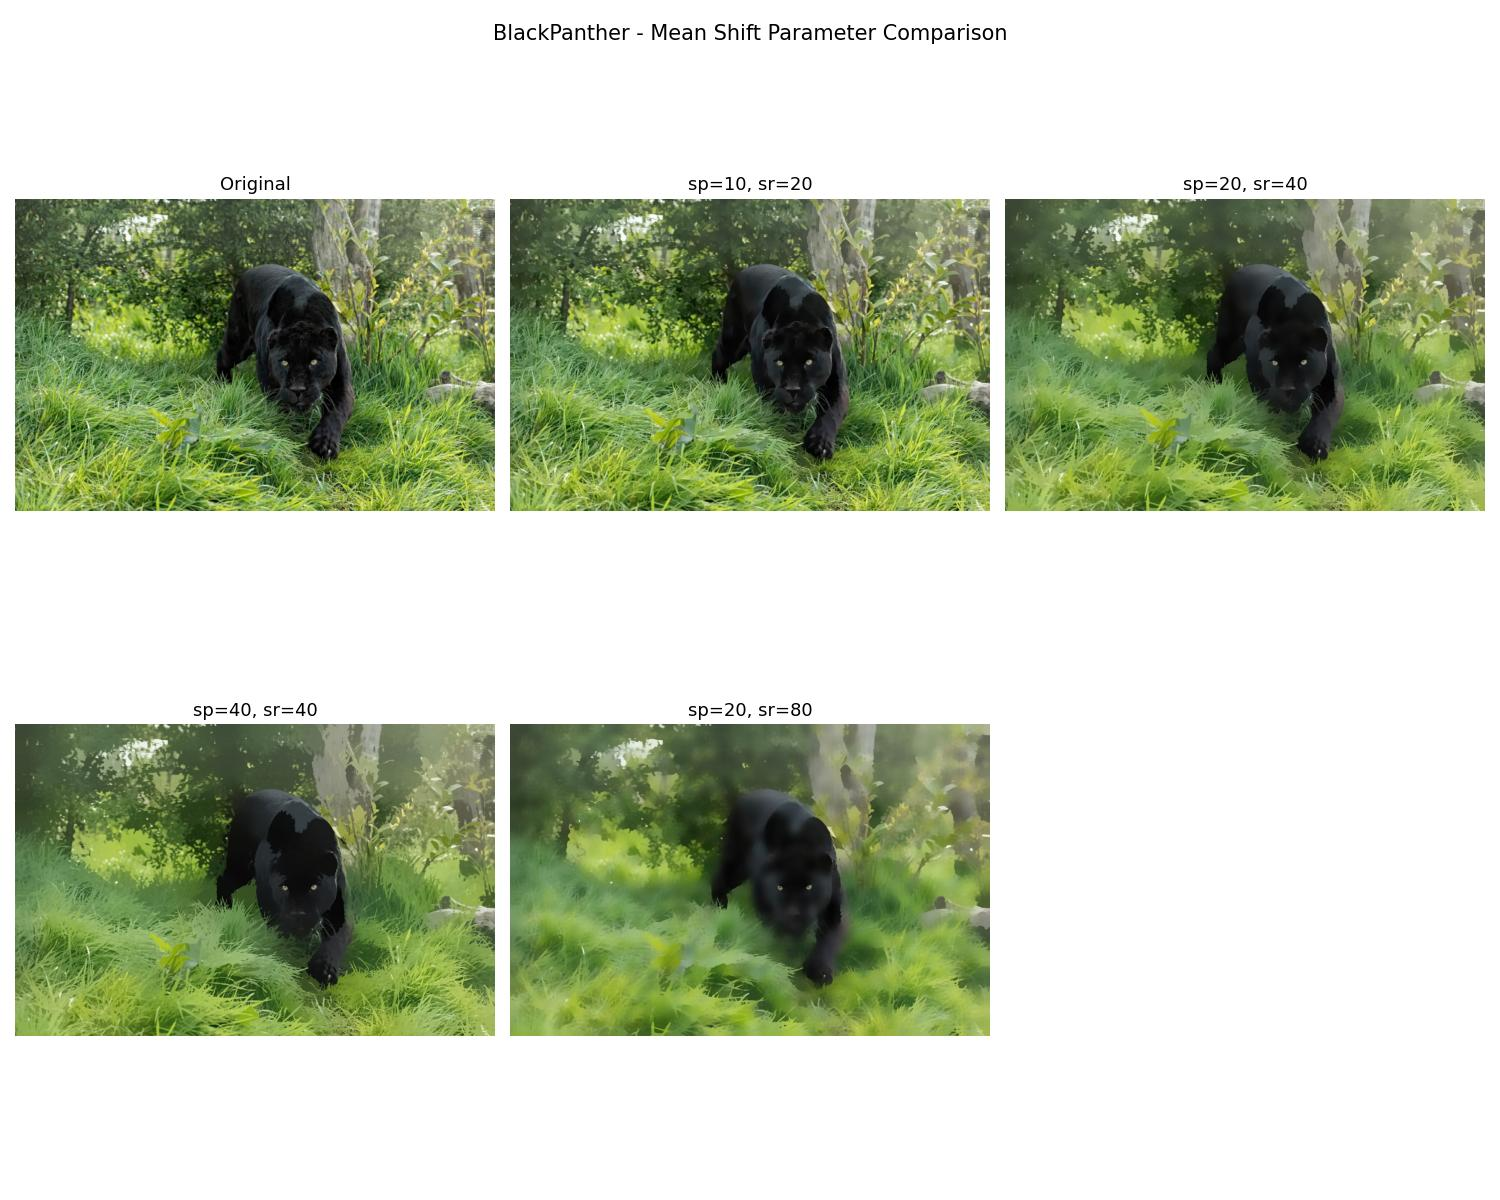
\includegraphics[width=\textwidth]{./images/Part_2/BlackPanther_MeanShift_comparison.jpg}
    \caption{مقایسه تاثیر پارامترهای مختلف الگوریتم \lr{Mean Shift} روی تصویر پلنگ سیاه. در حالت‌های با شعاع رنگی بسیار بالا، لبه‌های حیوان محو می‌شوند.}
    \label{fig:mean_shift_comparison}
\end{figure}

\clearpage
\begin{stepbox}
\field{پاسخ به سوال تمرین: حد فاصله همگرایی و حساسیت الگوریتم}{
حد فاصله‌ای که نقاط همگرایی بر اساس آن متمایز تلقی می‌شوند، در پارامتر \lr{\texttt{term\_crit}} تعیین می‌گردد. در این پیاده‌سازی، این حد فاصله (یا \lr{Epsilon}) برابر با \textbf{۱ پیکسل} در نظر گرفته شده است.

\textbf{میزان حساسیت الگوریتم:} این الگوریتم به شدت نسبت به این پارامتر حساس است:
\begin{itemize}
    \item اگر حد فاصله بسیار کوچک انتخاب شود (مثلاً 0.1)، الگوریتم به تغییرات بسیار ریزِ رنگی حساس شده و وسواس زیادی به خرج می‌دهد؛ این امر باعث افزایش چشمگیر زمان اجرا و بروز پدیده‌ی بیش‌بخش‌بندی (\lr{Over-segmentation}) می‌شود.
    \item در مقابل، اگر این حد فاصله بزرگ در نظر گرفته شود (مثلاً 5)، توقف زودهنگام رخ داده (\lr{Under-segmentation}) و بافت‌ها به خوبی در خوشه‌های یکپارچه ترکیب نمی‌شوند.
\end{itemize}
}
\end{stepbox}

\begin{tipbox}[بهینه‌سازی زمان اجرا]
از آنجایی که الگوریتم \lr{Mean Shift} محاسبات سنگینی دارد، استفاده از یک سقف برای حداکثر تعداد تکرار (در اینجا شرط \lr{MAX\_ITER = 5}) در کنار شرطِ حد فاصله‌ی همگرایی، از اجرای حلقه‌های طولانی و بی‌نهایتِ احتمالی جلوگیری می‌کند.
\end{tipbox}